\section{Hyphal Grafting and Deep Composition Contracts}

Complex ARC reasoning rules rarely arise as atomic primitives; they are formed by composing modular operators such as connected component extractors, spatial transformers, and stencil stampers. We formalize this composition through the biological metaphor of \textit{hyphal grafting}.

\subsection{Static Preflight Subtype Checking}
Let $A$ and $B$ denote two transformation nodes encapsulated within parametric types:
\begin{equation}
A :: \texttt{GraftNode}\{\mathrm{In}_A, \mathrm{Out}_A\}, \quad B :: \texttt{GraftNode}\{\mathrm{In}_B, \mathrm{Out}_B\}
\end{equation}
Before connecting $A$ and $B$, the system evaluates Julia's subtype lattice relation:
\begin{equation}
\mathrm{Out}_A <: \mathrm{In}_B
\end{equation}
If this condition is violated, the edge is rejected during preflight validation with zero executions of the underlying functions $A.f$ or $B.f$. This resolves a significant source of latency in large search graphs by pruning invalid compositional branches before dispatch.

\subsection{Runtime Intermediate Boundary Enforcement}
Static subtyping guarantees that declared signatures are compatible; however, it does not guarantee that an arbitrary implementation $A.f$ strictly respects its declared return type for all edge cases. To prevent unverified types from propagating across intermediate pipeline boundaries, the composed execution wrapper is defined as:
\begin{equation}
(B \circ A)(x) = B(A(x))
\end{equation}
where each node call wrapper $(N)(x)$ enforces:
\begin{equation}
\texttt{Core.typeassert}(N.f(x), \mathrm{Out}_N)
\end{equation}
This ensures that any intermediate contract violation immediately triggers an auditable \texttt{TypeError} at the exact boundary of failure, rather than corrupting subsequent pipeline stages.

\begin{figure}[htbp]
  \centering
  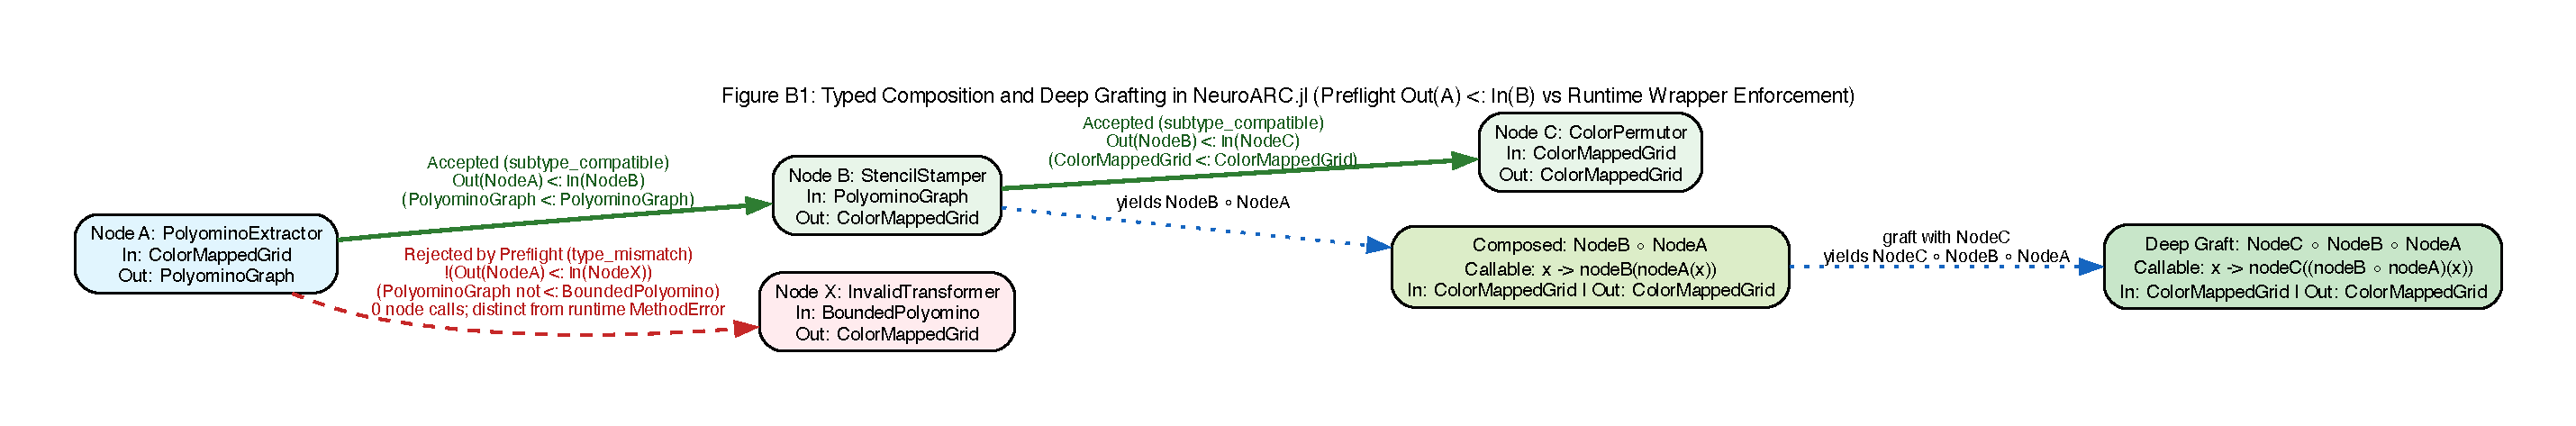
\includegraphics[width=\textwidth]{figures/figure_b1_typed_grafting.pdf}
  \caption{\textbf{Figure B1: Typed Composition and Deep Grafting Contract.} Illustrates preflight compatibility checking ($\mathrm{Out}(A) <: \mathrm{In}(B)$), typed verdicts (\texttt{Accepted} vs \texttt{Rejected}), associative three-stage deep grafting ($C \circ B \circ A$), and runtime intermediate boundary type assertions.}
  \label{fig:typed_grafting}
\end{figure}
